  %# -*- coding: utf-8-unix -*-
%%==================================================
%% chapter04.tex for SJRU Master Rhesis
%% distributed
%%==================================================
%\bibliographystyle{sjtu2}%[此处用于每章都生产参考文献]

% equation有编号 displaymath无编号

\chapter{基于分布式处理相似轨迹查询}
\label{chap:distributed}

\section{大规模数据集群处理}
\label{sec:bigdata-intro}
集群计算随着如今海量数据的发展在许多领域都有着广泛应用,以高效准确完成大量数据并行级的处理任务。集群计算需要提供本地化任务规划、高容错机制和数据负载平衡基本功能。除此之外,集群计算中我们也会关注某一个数据集运用在并行操作去完成指定目标任务。\emph{MapReduce}是目前分布式处理或并行计算常用的大规模数据处理和生成的编程模型。其工作的大致思路在于用户自定义合适的$map$函数去处理初步输入的键值对数据并产生中间键值对结果,之后定义$reduce$函数将中间结果以相同的关键字进行合并生成最终的结果。

对于数据密集型的应用而言,可扩展的分布式系统对于系统运行和数据处理都有着很重要的帮助。合理的分布式系统可以为系统提供在通用硬件上运行时的容错保护,并且能保证多用户请求的高度并行处理。\emph{Hadoop}分布式文件系统(\emph{HDFS})借鉴了\emph{Google}文件系统(\emph{GFS})的大部分设计架构并实现了高度的容错保护机制并且能良好地运行于廉价的硬件设备之上。与此同时,HDFS也保证了在应用中数据的高度吞吐速率,使得HDFS能高效运行具有很大数据集的任务或应用。

\subsection{Spark处理引擎简介}
\label{subsec:spark}
\emph{MapReduce}变成模型和\emph{HDFS}可在大规模数据密集型应用良好,但对于一些需要重复使用中间数据或需要暂时保留中间数据的应用处理中,之前常用的集群计算模型\emph{Hadoop}由于需要将中间数据读写与\emph{HDFS}中从而产生了中间读写时间浪费,从而影响了应用性能。基于这一点,\emph{Spark}作为在主流针对大规模数据处理的集群计算模型之一,在保证之前集群计算模型功能的同时,使用一种名为弹性分布式数据集(\emph{Resilient Distributed Datasets})的抽象,使得其可以将集群任务中的中间结果保存于设备的内存之中,以便之后的读写操作。因此,在大数据挖掘领域中,\emph{Spark}能够比\emph{Hadoop MapReduce}能为高效的处理需要迭代数据的集群计算。

\subsection{弹性分布数据集RDD}
\label{subsec:rdd}
\emph{Spark}集群计算处理引擎与之前集群处理的主要不同点即在于其引入的弹性分布式数据集(\emph{RDD})这一抽象概念。这一分布式内存抽象使得用户或程序员可以在容错机制的保护下在大规模集群设备中运行基于内存的数据操作。\emph{RDD}高效处理大数据在应用中的重用问题,作为一个并行的数据结构可以方便用户在内存中处理集群计算的中间过程数据,因地制宜分割数据集以更合理将任务分配个对应的工作节点,再结合丰富的内定操作函数以快速处理数据。
而\emph{RDD}提供的生成模式也能为我们设计算法提供更多思路。\emph{RDD}可以通过$parallelize$函数将程序中已有的数据用于生成为\emph{RDD},或通过对例如\emph{HDFS}、\emph{Hbase}等等的外部文件系统或外部数据源来生成\emph{RDD}。

\subsection{Spark Standalone集群模式}
\label{subsec:standalone}
\emph{Spark}应用在集群模式运营中运行独立的进程组,通过驱动程序中的\emph{Spark}上下文变量\emph{SparkContext}来设定运行参数和初始化。运行过程主要根据\emph{SparkContext}来连接如图\ref{fig:4-1}中具体不同种类的集群管理类型,并通过内定的\emph{Cluster Manager}来分配应用的资源获取。初始化成功后,\emph{Spark}通过获取集群节点上的执行进程并准备开始执行操作和处理数据。之后,\emph{Spark}会将应用代码分发给各个节点并使之运行。

\begin{figure}[!htp]
  \centering
  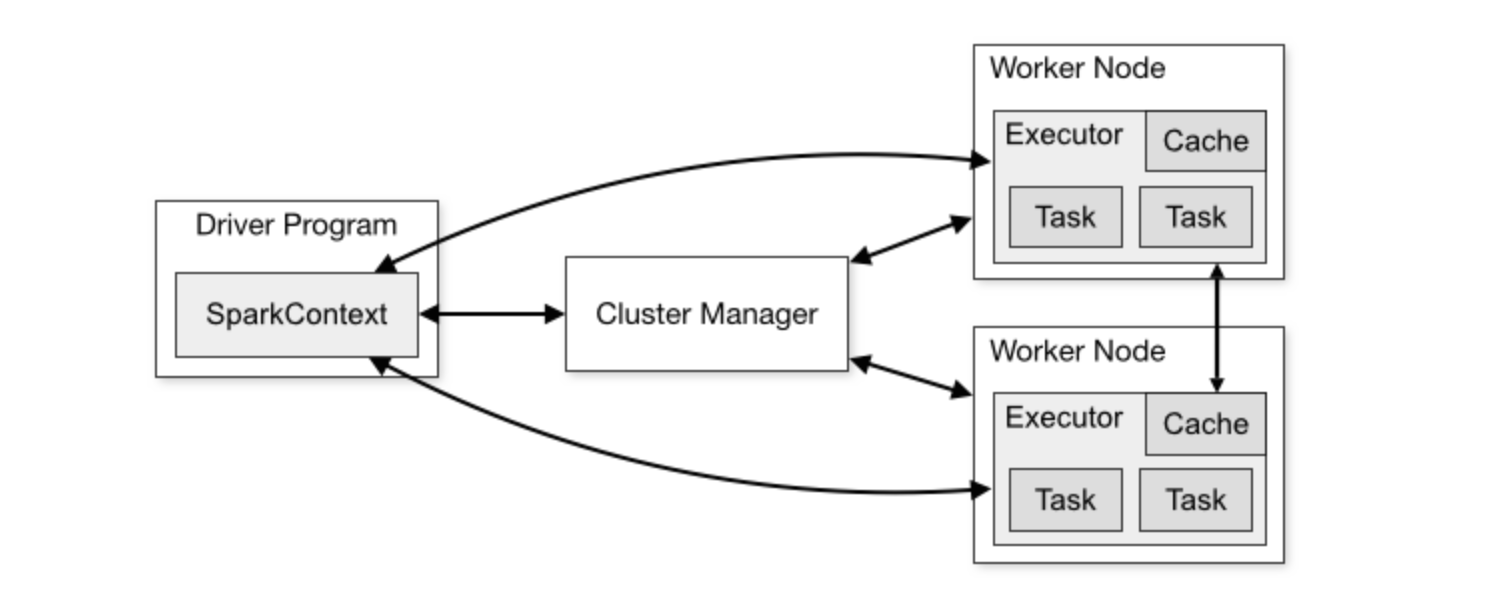
\includegraphics[width=0.6\textwidth]{chapter04/clustermanager.png}
  \bicaption[fig:4-1]{这里将出现在插图索引中}{集群管理大致模式}{Fig}{Cluster Managing Mode}
\end{figure}

在相似轨迹获取这一应用中,根据我们的应用场景和硬件设置,我们采用\emph{Spark}自带的\emph{Standalone}集群模式,其大致设计框架如图\ref{fig:4-2}所示。

\begin{figure}[!htp]
  \centering
  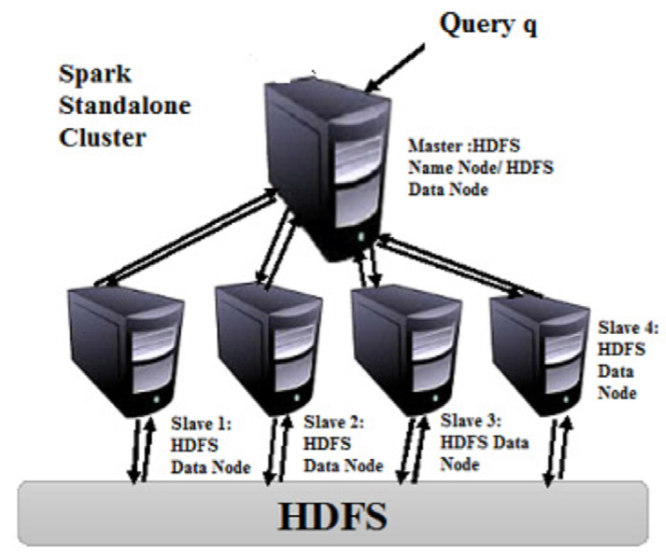
\includegraphics[width=0.5\textwidth]{chapter04/standalone.png}
  \bicaption[fig:4-2]{这里将出现在插图索引中}{Spark Standalone集群结构}{Fig}{Spark Standalone Architecture}
\end{figure}

在\emph{Standalone}集群模式中,我们通过一个在\emph{Spark}分布式环境下的简要集群管理者来简单建立集群处理环境。在这一集群环境中,主节点(\emph{Master Node})为驱动程序运行的设备节点。驱动程序不仅是与用户交互信息的接口(\emph{interface})程序,也负责分布式运行在\emph{Spark}环境中进程的运行情况。子节点们(\emph{Slave Nodes})为启动在工作节点中的进程提供运行环境,这些进程运行任务代码并在内存或磁盘中储存数据。在相似轨迹搜索中,我们将轨迹数据和预处理好的轨迹索引R树结构存储在\emph{HDFS}上,集群环境中的工作节点可以通过设定好的参数无需秘钥的共享\emph{HDFS}上已存储好的数据,这样,我们可以将相似轨迹搜索任务进一步以分布式的方法进行处理。

%\begin{figure}[!htp]
%  \centering
%  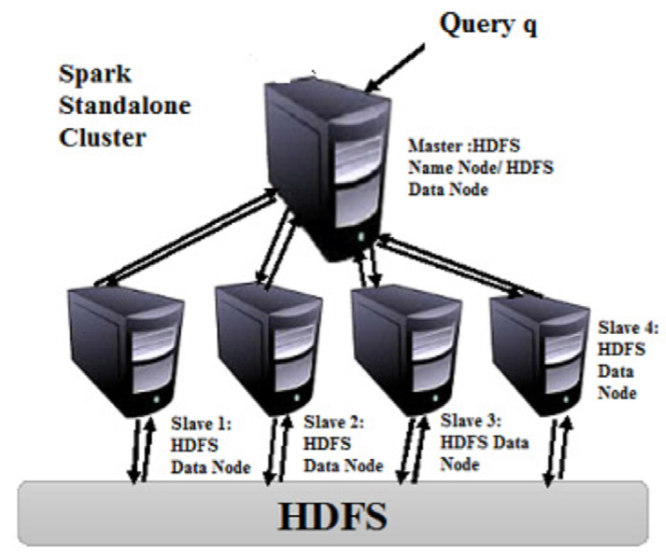
\includegraphics[width=0.5\textwidth]{chapter04/standalone.png}
%  \bicaption[fig:4-2]{这里将出现在插图索引中}{Spark Standalone集群结构}{Fig}%{Spark Standalone Architecture}
%\end{figure}


\section{分布式相似轨迹查询算法实现}
\label{sec:distributed algo}
在之前的工作描述中,我们对于相似轨迹查询的实现总会提及查询点集的数目相对较少这一前提。对于单机处理而言,如果将一整条轨迹的轨迹数据点作为输入或者查询点集过多,由于增长型k最近邻查询会对每一个查询点都进行$\lambda$-NN的搜索处理,因此整个相似轨迹的查询过程会显得相对缓慢。但有些时候,将一条轨迹作为相似轨迹查询的输入的确更简单且更人性化。在硬件设置对算法性能的约束下,借助基于地理位置点的轨迹简化方法,我们可以对前一章所涉及的相似轨迹查询方法通过加入\emph{Spark}分布式集群处理的手段,做到以一条轨迹为输入的相似轨迹查询操作。

\subsection{基于地理位置点的轨迹简化方法}
\label{subsec:trajectory simplification based on locations}
轨迹简化在本文中是比较重要的预处理过程。在保证轨迹数据可用性的同时也能压缩了原始轨迹数据的大小,可以在存储空间和搜索时间给予算法改善。在本文中,主要采用语义相关的轨迹简化算法,称为$TS$ $algorithm$(TS),它主要思路一条轨迹中重要的或具有特定语义的轨迹点从而进行压缩。TS轨迹简化算法既保证了轨迹的大致路线也保留了重要的特定轨迹点。基于轨迹点的相似轨迹查询用户大概率会使用一些在地理意义上重要的轨迹点,因此选择基于地理语义的轨迹压缩方法能够将轨迹简化结果和相似轨迹查询匹配使用。

该算法\ref{algo:ts}主要分为四个过程:分段、段权值排序、点权值计算和点选择。由于本工作数据集只针对车载轨迹数据,则在第一步只用进行简单的分段操作而不用进行轨迹类型分类操作。而第二步根据设定参数求出每一段的权值并通过算法定义参数保留段轨迹语义。第三步计算每个数据点的权值并通过正则化决定每一段子轨迹内选择保留相对比例的数据点。最后选择符合算法条件的点作为简化结果返回。
\\

\begin{algorithm}
% \begin{algorithm}[H] % 强制定位
\caption{轨迹简化(Trajectory Simplification)算法}
\label{algo:ts}
\begin{algorithmic}[1] %每行显示行号
\Require 一条原始轨迹数据$Traj$, 简化后轨迹点数目$m$ % 输入
\Ensure 一条简化后只有$m$个点的轨迹$Traj'$ % 输出

\State $Traj' \gets \emptyset$
\State $Seg[] \gets Segmentation(Traj)$ //将轨迹Traj分段
\State DistributePoints(Seg[], m);	//求段权值并参数初始化
\For{Each Segment $s$ in $Seg[]$}	
	\State WeightPoints($s$)	//求点权值
    \State $s'$ $\gets$ SelectPoints($s$)	//选择点组成新的轨迹段
    \State $Traj'$ $\gets$ $Traj \cup s'$	//合并新轨迹段组成结果
  \EndFor
\end{algorithmic}
\end{algorithm}

\subsection{Spark分布式相似轨迹查询}
\label{subsec:dis algo similar traj}